\chapter{Centrality measures}
\section{Some famous centrality measures}
The centrality of a node is a common problem of various fields such as biology, computer science, sociology, psychology. There are some old and popular measures to compute the centrality:
\begin{itemize}
	\item Closeness
	\item Betweenness
\end{itemize}
Next we examine some algorithms for computing them
\section{Closeness}
\subsection{Definition}
In words, the closeness says how a node is distant from the other nodes.\\
The formula for calculate is:
\begin{align*}
c(v) = \dfrac{n-1}{\sum_{u \in V} d(v,u)}
\end{align*}
A variant of this definition for non strongly connected components is
\begin{align*}
c(v)  = \dfrac{r(v) -1}{f(v)} \dfrac{r(v)-1}{n-1} = \dfrac{(r(v) - 1)^2}{(n-1)f(v)}
\end{align*}
 where $ r(v) $ is the set of reachable nodes from v. If the graph is strongly connected we have the previous definition, in fact
 \begin{align*}
 	\dfrac{(n - 1)^2}{(n-1)f(v)} = \dfrac{n-1}{f(v)}
 \end{align*}
 \subsection{A simple approach}
 The initial idea for computing the closeness is doing a BFS from all nodes to obtain all the distances but this have time complexity $ O(nm) $ which is too much for real graph.
 \section*{The pruned breadth first search}
  A similar problem is find the top k nodes with lower closeness but for doing this we need before the pruned breadth first search.\\
  \subsection{The upper bound on closeness}
 The pruned breadth first search use a lower bound on the farness of the nodes from v, that is equivalent to an upper bound of the closeness.\\
 Let's define the following terms:
 \begin{itemize}
 	\item $ \Gamma_d(v) = $ set of nodes at level \textit{d} of the BFS tree starting from \textit{v}
 	\item $ \gamma_d(v) = |\Gamma_d(v)| $
 	\item $ f_d(v) = \sum_{i=1}^{d} i \cdot \gamma_i(v) $
 	\item $ n_d(v) = \sum_{i=1}^{d} \gamma_i(v) $
\end{itemize}
Now let's define a lower bound on closeness:
\begin{center}
	$ f(v) \geq f_d(v) + (d+1) \cdot  \gamma_{d+1}(v) + (d+2)(r(v) - n_{d+1}(v))$
\end{center}
Since $ n_{d+1}(v) = \gamma_{d+1}(v) + n_d(v) $ we have
\begin{align*}
	 f(v) &\geq f_d(v) + (d+1) \cdot \gamma_{d+1}(v) + (d+2)\left[r(v) - (\gamma_{d+1}(v) + n_d(v))\right] \\
	 &= f_d(v) + (d+1) \cdot \gamma_{d+1}(v) - (d+2) \cdot \gamma_{d+1}(v) + (d+2)(r(v) - n_d(v)) \\
	 &= f_d(v)   - \gamma_{d+1}(v) + (d+2)(r(v) - n_d(v)) 
\end{align*}
We must consider that at the level \textit{d} we don't know how much is $ \gamma_{d+1}(v) $ so we use an upper bound that is the sum of degree of nodes on level \textit{d}:
\begin{align*}
	\gamma_{d+1}(v) \leq \sum_{u \in \Gamma_d(v)} degree(u) := \tilde{\gamma}_{d+1}(v)
\end{align*}
So we use the latter approximation on lower bound of farness $ f(v) $ 
\begin{align*}
	 f(v) &\geq \tilde{f}_d(v, r(v)) :=  f_d(v)   - \tilde{\gamma}_{d+1}(v) + (d+2)(r(v) - n_d(v))
\end{align*}
that is equivalent to an upper bound on closeness:
\begin{align*}
	c(v) \leq \dfrac{\left[r(v) - 1 \right]^2}{(n-1) \cdot  \tilde{f}_d(v, r(v)) } := \tilde{c}_d(v) 
\end{align*}
\subsubsection{How to prune the breadth first search}
The pruned breadth first search receive in input the following arguments:
\begin{itemize}
	\item \textit{v}: the starting node of pruned BFS
	\item $ x_k $: the k-th biggest closeness value found until now (0 if not are processed at least k vertices)
\end{itemize}
then at each level \textit{d} of \textit{BFS} tree we check if $ x_k >  \tilde{c}_d(v)  \geq c_d(v)  $, and, if it is true, it means that it is not in the \textit{k} lowest values of closeness in the graph, so we can stop the \textit{BFS}.
\subsection{Compute the upper bound on closeness}
Once we have defined the algorithm in the latter section, then it remains one thing: calculate $ r(v) $ for each node.\\
We have four different cases:
\begin{itemize}
	\item Graph indirected and strongly connected: $ r(v) \rightarrow n \,\,\forall v \in V $
	\item  Graph indirected but not strongly connected: A linear time scan graph is needed then set $ r(v) = |SCC| : v \in SCC \,\, \forall v \in V $ that mean set $ r(v) $ to the size of strongly connected component where it belongs
	\item Graph directed and strongly connected :  $ r(v) \rightarrow n \,\,\forall v \in V $
	\item Graph directed but not strongly connected : see below
\end{itemize}
\subsubsection{Graph directed but not strongly connected}
Suppose that $ r(v) $ is included in the range $ [\alpha(v) , \omega(v)] $ a lower bound for $ \dfrac{1}{c(v)} $ is obtained simply bi reverting the upper bound in the latter section:
\begin{align*}
 \dfrac{1}{c(v)} \geq \dfrac{(n-1) \cdot \tilde{f}_d(v, r(v))}{(r(v) -1)^2}
\end{align*}
Then if we define $ a = d+2  $ and $ b = \tilde{\gamma}_{d+1}(v) + a(n_d(v) -1) - f_d(v) $ we have that
\begin{align*}
	f(v) \geq \tilde{f}_d(v, r(v)) &=  f_d(v)   - \tilde{\gamma}_{d+1}(v) + (d+2)(r(v) - n_d(v)) \\
	&=  f_d(v)   - \tilde{\gamma}_{d+1}(v) + a \cdot (r(v) - n_d(v)) \\
	&=  f_d(v)   - \tilde{\gamma}_{d+1}(v) + a \cdot (r(v) - n_d(v) + 1 - 1) \\
	&=  f_d(v)   - \tilde{\gamma}_{d+1}(v) + a \cdot (r(v) - 1))  - a \cdot n_d(v) + a\\
	&=  f_d(v)   - \tilde{\gamma}_{d+1}(v) + a \cdot (r(v) - 1))  + a (-  n_d(v) + 1)\\
	&=  a \cdot (r(v) - 1))   - \tilde{\gamma}_{d+1}(v)   - a (  n_d(v) -1)  + f_d(v)\\
	&= a \cdot (r(v) - 1))   - b
\end{align*}

so we can write the lower bound as 
\begin{align*}
\dfrac{1}{c(v)} \geq \dfrac{(n-1) \cdot \tilde{f}_d(v, r(v))}{(r(v) -1)^2} =(n-1)\dfrac{a \cdot (r(v) - 1))   - b}{(r(v) -1)^2}
\end{align*}
Now consider the functions in the form $ g(x) = \dfrac{ax - b}{x^2} $ and the derivative $ g'(x) = \dfrac{-ax + 2b}{x^3} $: we can easily see that we have a zero in the derivative with $ x = \dfrac{2b}{a} $ and it is a local maximum because x is positive in range $ 0 < x < \frac{2b}{a} $ and negative in $ x > \frac{2b}{a} $. Then this it implies that for $ x > 0 $ there aren't local minimum so for any interval $ [x_1, x_2] $ the local minimum in the interval is $ x_1  $ or $ x_2 $ that in formula is $ \forall x \in [x_1, x_2] \,\, g(x)  \geq \min(g(x_1), g(x_2))$
\begin{figure}[H]
	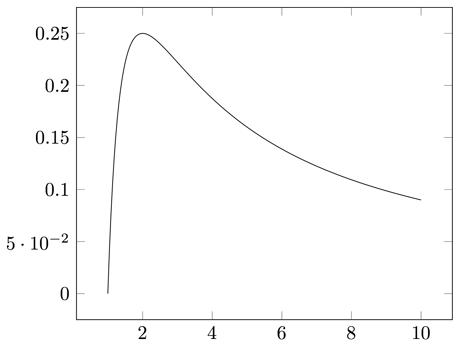
\includegraphics[width=0.7\linewidth]{img/local_maximum}
	\caption{Plot of $ g(x) = \dfrac{ax -b}{x^2} $ with $ a = b = 1 $}
	\label{fig:localmaximum}
\end{figure}
Returning to the lower bound of $ \frac{1}{c(v)} $ we can use the same reasoning with $ (n-1)\dfrac{a \cdot (r(v) - 1))   - b}{(r(v) -1)^2} $ so we can say that 
\begin{align*}
\dfrac{1}{c(v)} \geq (n-1) \cdot \dfrac{\tilde{f}_d(v, r(v))}{(r(v) -1)^2} \geq (n-1) \cdot \min\left( \dfrac{\tilde{f}_d(v, \alpha(v))}{(\alpha(v) -1)^2}, \dfrac{\tilde{f}_d(v, \omega(v))}{(\omega(v) -1)^2} \right)
\end{align*}

\subsection{Compute $ \alpha(v) \text{ and }  \omega(v) $}